\hypertarget{appendix-932cf7182ff1}{}
\section*{08 - Linear Algebra - Visual Recall}
\section{Phase 8 --- Linear Algebra: Active Recall}\label{phase-8-linear-algebra-active-recall}

\textbf{Fast spine:} Measurements constrain → rank separates knowledge from freedom → factorizations expose structure → eigenvectors describe square-map directions → SVD describes every map → stable APIs report evidence.

Read the full explanations in \href{Continuous\%20Notes/Computing\%20Foundations\%20-\%20From\%20Bits\%20to\%20C++\%20and\%20Systems\%20APIs\#The\%20graphics\%20problem\%20hiding\%20inside\%20a\%20matrix\%20equation}{From Constraints to Spectra}. These figure links jump to their source chapters.

\subsection{The story at a glance}\label{the-story-at-a-glance}

\pandocbounded{\includegraphics[keepaspectratio,alt={Diagram}]{/Users/swayamsingal/Library/Mobile Documents/iCloud~md~obsidian/Documents/Master/Book Production/AllMight Codex/QA/print-reference-dedup/assets/print/f9dec25434c3fe1a6fe55360c13433c0ea403b0d18f8d618dd5defe53257313e.pdf}}

\subsection{Retrieve the mechanisms}\label{retrieve-the-mechanisms}

{\def\LTcaptype{none} % do not increment counter
\begin{longtable}[]{@{}
  >{\raggedright\arraybackslash}p{(\linewidth - 4\tabcolsep) * \real{0.3333}}
  >{\raggedright\arraybackslash}p{(\linewidth - 4\tabcolsep) * \real{0.3333}}
  >{\raggedright\arraybackslash}p{(\linewidth - 4\tabcolsep) * \real{0.3333}}@{}}
\toprule\noalign{}
\begin{minipage}[b]{\linewidth}\raggedright
Cue
\end{minipage} & \begin{minipage}[b]{\linewidth}\raggedright
Short answer
\end{minipage} & \begin{minipage}[b]{\linewidth}\raggedright
Read / view
\end{minipage} \\
\midrule\noalign{}
\endhead
\bottomrule\noalign{}
\endlastfoot
Why may \(A\mathbf x=\mathbf b\) have no answer? & The target is outside \(\operatorname{Col}(A)\). & \href{Continuous\%20Notes/Computing\%20Foundations\%20-\%20From\%20Bits\%20to\%20C++\%20and\%20Systems\%20APIs\#A\%20linear\%20equation\%20is\%20a\%20measurement,\%20and\%20several\%20equations\%20are\%20geometry/}{Constraint geometry} · \href{Continuous\%20Notes/Computing\%20Foundations\%20-\%20From\%20Bits\%20to\%20C++\%20and\%20Systems\%20APIs\#Figure\%20L2\%20-\%20Consistency,\%20freedom,\%20and\%20the\%20four\%20fundamental\%20spaces/}{L2} \\
What does a null vector mean? & An input change no measurement can see; add it to any solution. & \href{Continuous\%20Notes/Computing\%20Foundations\%20-\%20From\%20Bits\%20to\%20C++\%20and\%20Systems\%20APIs\#Rank\%20separates\%20what\%20the\%20measurements\%20determine\%20from\%20what\%20they\%20leave\%20free/}{Four spaces} · \href{Continuous\%20Notes/Computing\%20Foundations\%20-\%20From\%20Bits\%20to\%20C++\%20and\%20Systems\%20APIs\#Figure\%20L2\%20-\%20Consistency,\%20freedom,\%20and\%20the\%20four\%20fundamental\%20spaces/}{L2} \\
What does elimination preserve? & The solution set, only if row operations also transform \(\mathbf b\). & \href{Continuous\%20Notes/Computing\%20Foundations\%20-\%20From\%20Bits\%20to\%20C++\%20and\%20Systems\%20APIs\#Elimination\%20turns\%20the\%20geometry\%20into\%20an\%20auditable\%20calculation/}{Elimination} · \href{Continuous\%20Notes/Computing\%20Foundations\%20-\%20From\%20Bits\%20to\%20C++\%20and\%20Systems\%20APIs\#Figure\%20L3\%20-\%20Elimination\%20stores\%20work\%20for\%20later\%20solves/}{L3} \\
Why factor once? & Reuse \(L,U\) or \(Q,R\) for additional right-hand sides. & \href{Continuous\%20Notes/Computing\%20Foundations\%20-\%20From\%20Bits\%20to\%20C++\%20and\%20Systems\%20APIs\#Figure\%20L3\%20-\%20Elimination\%20stores\%20work\%20for\%20later\%20solves/}{L3} \\
Which factorization for what structure? & LU general square; Cholesky SPD; QR least squares; SVD rank insight; iteration for huge sparse systems when suitable. & \href{Continuous\%20Notes/Computing\%20Foundations\%20-\%20From\%20Bits\%20to\%20C++\%20and\%20Systems\%20APIs\#Structure\%20makes\%20a\%20decomposition\%20a\%20better\%20tool\%20than\%20generic\%20elimination/}{Factorization guide} · \href{Continuous\%20Notes/Computing\%20Foundations\%20-\%20From\%20Bits\%20to\%20C++\%20and\%20Systems\%20APIs\#Figure\%20L4\%20-\%20Matrix\%20structure\%20determines\%20the\%20useful\%20factorization/}{L4} \\
What does a small residual prove? & Near satisfaction of the equations; sensitivity can still make the solution inaccurate. & \href{Continuous\%20Notes/Computing\%20Foundations\%20-\%20From\%20Bits\%20to\%20C++\%20and\%20Systems\%20APIs\#Eigenvectors\%20reveal\%20the\%20directions\%20a\%20square\%20map\%20does\%20not\%20turn/}{Eigenpair sensitivity} · \href{Continuous\%20Notes/Computing\%20Foundations\%20-\%20From\%20Bits\%20to\%20C++\%20and\%20Systems\%20APIs\#Matrix\%20norms\%20give\%20scale\%20to\%20residuals\%20and\%20error\%20claims/}{Norms and error} \\
Why is a symmetric eigenbasis special? & It is orthonormal, preserving 2-norm while diagonalizing the map. & \href{Continuous\%20Notes/Computing\%20Foundations\%20-\%20From\%20Bits\%20to\%20C++\%20and\%20Systems\%20APIs\#Figure\%20L5\%20-\%20Eigenanalysis\%20is\%20cleanest\%20when\%20the\%20basis\%20is\%20orthonormal/}{L5} \\
What is the SVD action? & Input orthogonal coordinates → independent stretches → output orthogonal coordinates. & \href{Continuous\%20Notes/Computing\%20Foundations\%20-\%20From\%20Bits\%20to\%20C++\%20and\%20Systems\%20APIs\#Singular\%20value\%20decomposition\%20covers\%20every\%20rectangular\%20map/}{SVD geometry} · \href{Continuous\%20Notes/Computing\%20Foundations\%20-\%20From\%20Bits\%20to\%20C++\%20and\%20Systems\%20APIs\#Figure\%20L6\%20-\%20Every\%20linear\%20map\%20is\%20orthogonal\%20change,\%20stretch,\%20orthogonal\%20change/}{L6} \\
What does the pseudoinverse choose? & Exact \(A^+\): least-squares fit, then minimum norm. Truncated \(A_\tau^+\): solve the retained-rank problem; original residual can increase. & \href{Continuous\%20Notes/Computing\%20Foundations\%20-\%20From\%20Bits\%20to\%20C++\%20and\%20Systems\%20APIs\#Pseudoinverse\%20makes\%20least\%20squares\%20and\%20minimum\%20norm\%20one\%20operation/}{Pseudoinverse} · \href{Continuous\%20Notes/Computing\%20Foundations\%20-\%20From\%20Bits\%20to\%20C++\%20and\%20Systems\%20APIs\#Figure\%20L7\%20-\%20The\%20singular\%20spectrum\%20makes\%20inversion\%20and\%20compression\%20explicit/}{L7} \\
How does PCA connect to SVD? & Center rows, factor \(X=U\Sigma V^\mathsf T\); \(V\) gives principal directions and \(U\Sigma\) scores. & \href{Continuous\%20Notes/Computing\%20Foundations\%20-\%20From\%20Bits\%20to\%20C++\%20and\%20Systems\%20APIs\#PCA\%20turns\%20a\%20cloud\%20of\%20points\%20into\%20measured\%20variation/}{PCA} \\
What does polar decomposition separate? & Orthogonal motion from symmetric stretch; reflection and singular ambiguity need attention. & \href{Continuous\%20Notes/Computing\%20Foundations\%20-\%20From\%20Bits\%20to\%20C++\%20and\%20Systems\%20APIs\#Polar\%20decomposition\%20separates\%20rotation-like\%20motion\%20from\%20stretch/}{Polar decomposition} \\
Which SVD checks are independent? & Reconstruction, \(U\) orthogonality, \(V\) orthogonality, ordering, dimensions, convergence. & \href{Continuous\%20Notes/Computing\%20Foundations\%20-\%20From\%20Bits\%20to\%20C++\%20and\%20Systems\%20APIs\#Figure\%20L8\%20-\%20SVD\%20validation\%20needs\%20independent\%20checks/}{L8} \\
When can diagonalization explain a matrix function? & When its eigenbasis is usable; otherwise use a stable function-specific algorithm. & \href{Continuous\%20Notes/Computing\%20Foundations\%20-\%20From\%20Bits\%20to\%20C++\%20and\%20Systems\%20APIs\#Matrix\%20functions\%20turn\%20repeated\%20linear\%20actions\%20into\%20one\%20operator/}{Matrix functions} · \href{Continuous\%20Notes/Computing\%20Foundations\%20-\%20From\%20Bits\%20to\%20C++\%20and\%20Systems\%20APIs\#Figure\%20L9\%20-\%20A\%20matrix\%20function\%20follows\%20the\%20same\%20action\%20after\%20a\%20change\%20of\%20basis/}{L9} \\
Direct or iterative solve? & Decide from size, sparsity, right-hand-side reuse, convergence, memory, and error needs. & \href{Continuous\%20Notes/Computing\%20Foundations\%20-\%20From\%20Bits\%20to\%20C++\%20and\%20Systems\%20APIs\#Figure\%20L10\%20-\%20Direct\%20and\%20iterative\%20methods\%20occupy\%20different\%20workloads/}{L10} \\
\end{longtable}
}

\subsection{Thirty-second reconstruction}\label{thirty-second-reconstruction}

\begin{enumerate}
\def\labelenumi{\arabic{enumi}.}
\tightlist
\item
  Sketch one measurement as a hyperplane; explain consistency using column space.
\item
  Explain why rank and nullity count determined and invisible directions.
\item
  Derive one pivot step and show the same row operation on the right-hand side.
\item
  Select LU, Cholesky, QR, SVD, or an iterative method from matrix structure.
\item
  Explain why normal equations square the condition number.
\item
  Trace \(A=U\Sigma V^\mathsf T\) on one vector.
\item
  State what thresholding changes in a pseudoinverse or truncated SVD.
\item
  Name separate SVD correctness checks and what a residual cannot prove.
\end{enumerate}

\href{Continuous\%20Notes/Computing\%20Foundations\%20-\%20From\%20Bits\%20to\%20C++\%20and\%20Systems\%20APIs\#The\%20graphics\%20problem\%20hiding\%20inside\%20a\%20matrix\%20equation}{Full teaching volume} · \href{}{100-part title ledger (01-Foundations-I, appendix-fd090d982a15 § Phase 8 - Parts 701-800)} · \hyperref[appendix-4ad47bdd269a]{Dependency spine}

\subsection{Fast retrieval: restore the details that are easy to blur}\label{fast-retrieval-restore-the-details-that-are-easy-to-blur}

\href{Continuous\%20Notes/Computing\%20Foundations\%20-\%20From\%20Bits\%20to\%20C++\%20and\%20Systems\%20APIs\#Figure\%20L6a\%20-\%20Watch\%20the\%20same\%20directions\%20become\%20an\%20ellipse}{Figure L6a: exact SVD geometry} · \href{Visual\%20Recall/phase8_svd_geometry.svg}{Editable SVG}

\begin{figure}
\centering
\pandocbounded{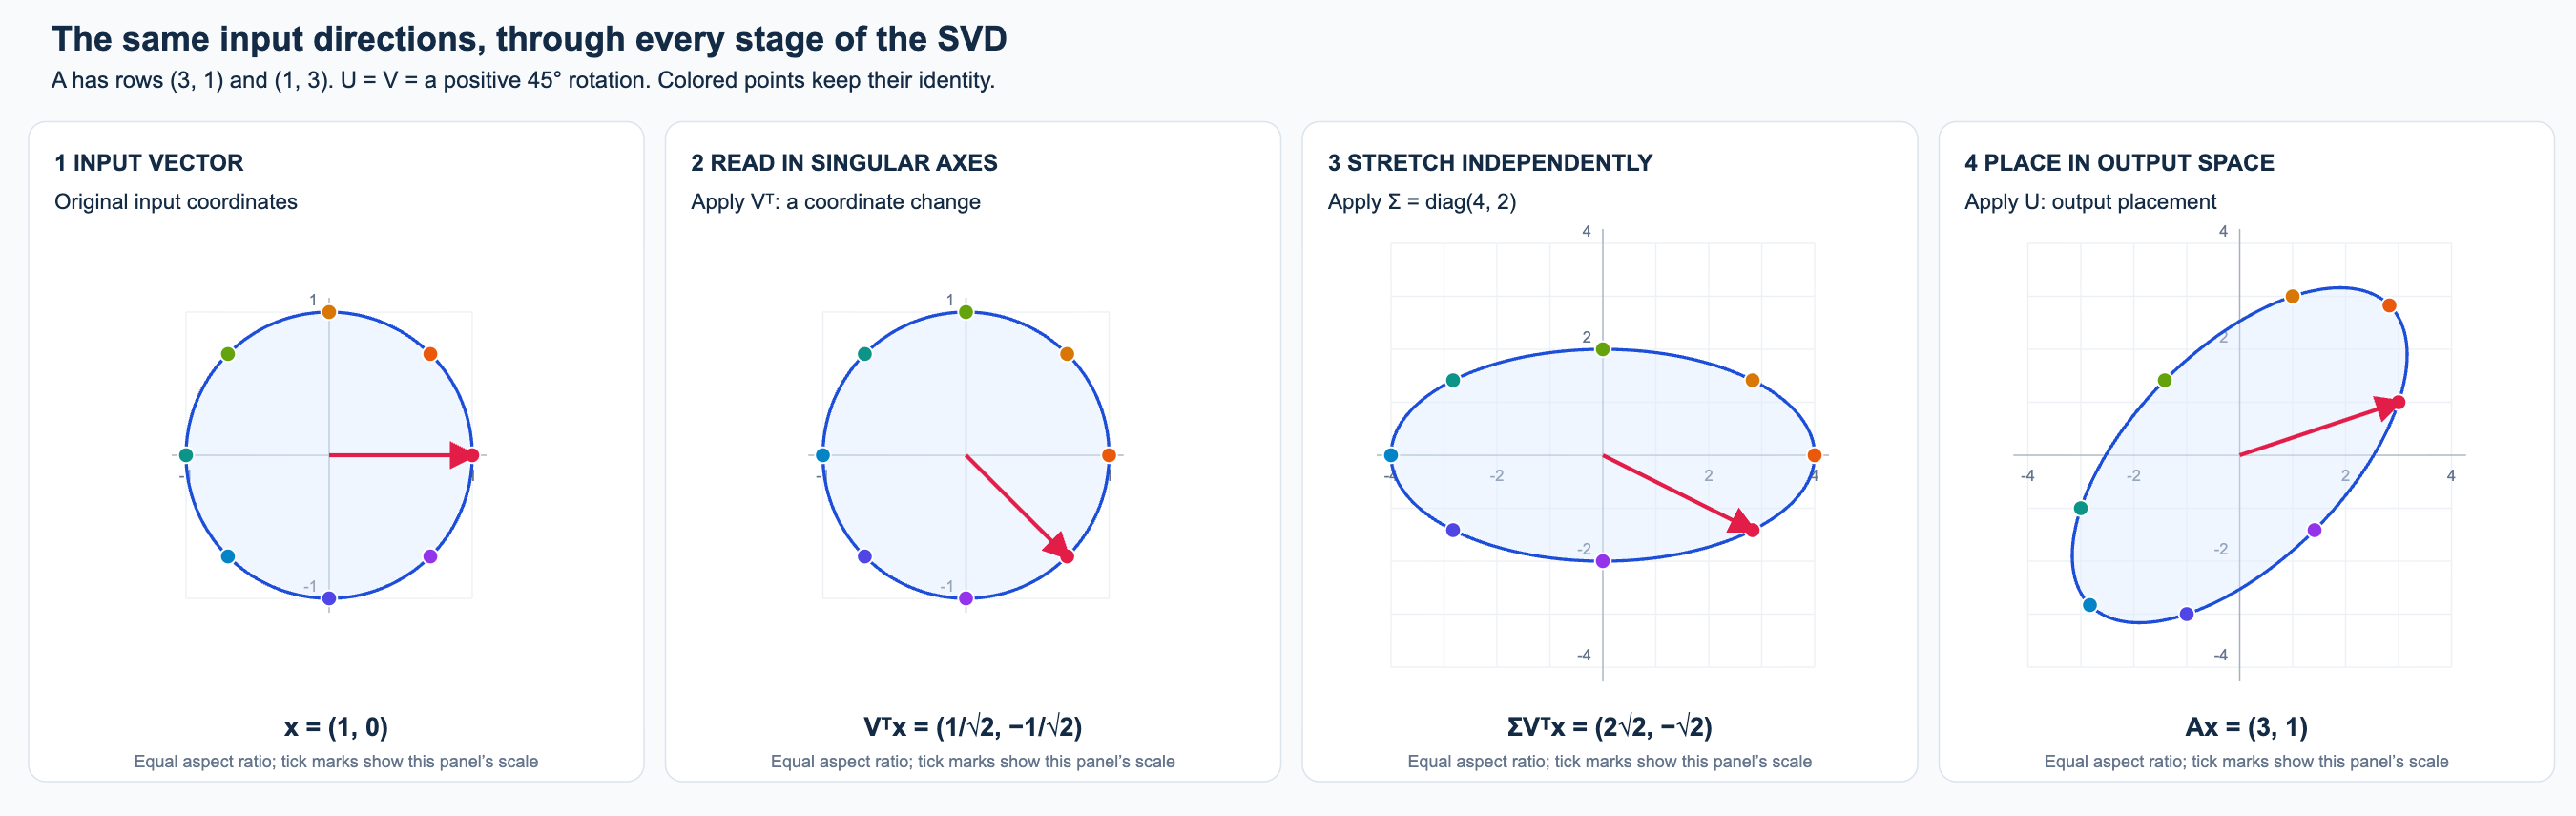
\includegraphics[keepaspectratio,alt={Visual Recall/phase8\_svd\_geometry.png}]{Visual Recall/phase8_svd_geometry.png}}
\caption{Visual Recall/phase8\_svd\_geometry.png}
\end{figure}

{\def\LTcaptype{none} % do not increment counter
\begin{longtable}[]{@{}
  >{\raggedright\arraybackslash}p{(\linewidth - 4\tabcolsep) * \real{0.3333}}
  >{\raggedright\arraybackslash}p{(\linewidth - 4\tabcolsep) * \real{0.3333}}
  >{\raggedright\arraybackslash}p{(\linewidth - 4\tabcolsep) * \real{0.3333}}@{}}
\toprule\noalign{}
\begin{minipage}[b]{\linewidth}\raggedright
Cue
\end{minipage} & \begin{minipage}[b]{\linewidth}\raggedright
Shortest reliable answer
\end{minipage} & \begin{minipage}[b]{\linewidth}\raggedright
Deep read / figure
\end{minipage} \\
\midrule\noalign{}
\endhead
\bottomrule\noalign{}
\endlastfoot
When does Gram--Schmidt normalize a new column? & Only if its residual norm is safely nonzero; rank deficiency needs rank handling or completion. & \href{Continuous\%20Notes/Computing\%20Foundations\%20-\%20From\%20Bits\%20to\%20C++\%20and\%20Systems\%20APIs\#Orthogonal\%20coordinates\%20preserve\%20the\%20shape\%20of\%20the\%20problem/}{Gram--Schmidt} \\
What does a Householder sign choice prevent? & Choose \(\alpha=-\operatorname{copysign}(\|x\|,x_1)\) to avoid cancellation; compute the norm safely. & \href{Continuous\%20Notes/Computing\%20Foundations\%20-\%20From\%20Bits\%20to\%20C++\%20and\%20Systems\%20APIs\#Reflections\%20and\%20plane\%20rotations\%20build\%20QR\%20without\%20losing\%20lengths/}{Householder reflectors} \\
When is Givens rotation undefined? & If \(a=b=0\), skip it; otherwise use \texttt{hypot(a,b)} for the scale. & \href{Continuous\%20Notes/Computing\%20Foundations\%20-\%20From\%20Bits\%20to\%20C++\%20and\%20Systems\%20APIs\#Reflections\%20and\%20plane\%20rotations\%20build\%20QR\%20without\%20losing\%20lengths/}{Givens rotations} \\
What residual remains after QR least squares? & The irreducible perpendicular part \(b_\perp=(I-QQ^T)b\); minimum residual norm is \(\|b_\perp\|\). & \href{Continuous\%20Notes/Computing\%20Foundations\%20-\%20From\%20Bits\%20to\%20C++\%20and\%20Systems\%20APIs\#QR\%20turns\%20least\%20squares\%20into\%20a\%20triangular\%20solve\%20plus\%20an\%20irreducible\%20residual/}{QR residual derivation} \\
What makes an eigenvector estimate sensitive? & A small residual is backward evidence; a small eigengap can still rotate the vector or subspace. & \href{Continuous\%20Notes/Computing\%20Foundations\%20-\%20From\%20Bits\%20to\%20C++\%20and\%20Systems\%20APIs\#Residuals\%20distinguish\%20backward\%20accuracy\%20from\%20forward\%20certainty/}{Residual and eigengap} · \href{Continuous\%20Notes/Computing\%20Foundations\%20-\%20From\%20Bits\%20to\%20C++\%20and\%20Systems\%20APIs\#Figure\%20L5\%20-\%20Eigenanalysis\%20is\%20cleanest\%20when\%20the\%20basis\%20is\%20orthonormal/}{L5} \\
What does a real Schur 2×2 block mean? & A real representation of a complex-conjugate eigenvalue pair; do not read only its diagonal. & \href{Continuous\%20Notes/Computing\%20Foundations\%20-\%20From\%20Bits\%20to\%20C++\%20and\%20Systems\%20APIs\#QR\%20iteration\%20and\%20Jacobi\%20rotations\%20preserve\%20the\%20spectrum\%20while\%20simplifying\%20shape/}{QR and Schur form} \\
Where is the plane-fit normal in an \(N\times3\) data SVD? & In the right singular vectors \(V\); take the smallest-variance direction. & \href{Continuous\%20Notes/Computing\%20Foundations\%20-\%20From\%20Bits\%20to\%20C++\%20and\%20Systems\%20APIs\#Plane\%20fits,\%20eigengaps,\%20and\%20interpretation\%20of\%20uncertain\%20components/}{Plane fit and eigengap} \\
What must a wide SVD return? & With \(r=\min(m,n)\), thin \(U:m\times r\), \(\sigma:r\), \(V^T:r\times n\); factor \(A^T\) if using a tall backend. & \href{Continuous\%20Notes/Computing\%20Foundations\%20-\%20From\%20Bits\%20to\%20C++\%20and\%20Systems\%20APIs\#Householder\%20reductions\%20turn\%20a\%20dense\%20SVD\%20into\%20a\%20bidiagonal\%20problem/}{Wide SVD shapes} · \href{Continuous\%20Notes/Computing\%20Foundations\%20-\%20From\%20Bits\%20to\%20C++\%20and\%20Systems\%20APIs\#Figure\%20L6\%20-\%20Every\%20linear\%20map\%20is\%20orthogonal\%20change,\%20stretch,\%20orthogonal\%20change/}{L6} \\
What are zero singular vectors for? & Right zero directions span \(\operatorname{Null}(A)\); full \(U\) zero/completion directions span \(\operatorname{Null}(A^T)\). & \href{Continuous\%20Notes/Computing\%20Foundations\%20-\%20From\%20Bits\%20to\%20C++\%20and\%20Systems\%20APIs\#Zero\%20singular\%20directions\%20require\%20deliberate\%20orthonormal\%20completion/}{Zero-singular completion} \\
What is the exact \(A^+\) rule? & Reciprocate every positive \(\sigma_i\); it minimizes original residual, then chooses minimum norm. & \href{Continuous\%20Notes/Computing\%20Foundations\%20-\%20From\%20Bits\%20to\%20C++\%20and\%20Systems\%20APIs\#The\%20Moore–Penrose\%20inverse\%20and\%20its\%20four\%20identities/}{Exact pseudoinverse} · \href{Continuous\%20Notes/Computing\%20Foundations\%20-\%20From\%20Bits\%20to\%20C++\%20and\%20Systems\%20APIs\#Figure\%20L7\%20-\%20The\%20singular\%20spectrum\%20makes\%20inversion\%20and\%20compression\%20explicit/}{L7} \\
What does \(A_\tau^+\) change? & It discards positive values at or below \(\tau\); the original least-squares residual can increase. & \href{Continuous\%20Notes/Computing\%20Foundations\%20-\%20From\%20Bits\%20to\%20C++\%20and\%20Systems\%20APIs\#Thresholding\%20and\%20regularization\%20are\%20different\%20choices/}{Thresholding versus regularization} · \href{Continuous\%20Notes/Computing\%20Foundations\%20-\%20From\%20Bits\%20to\%20C++\%20and\%20Systems\%20APIs\#Figure\%20L7\%20-\%20The\%20singular\%20spectrum\%20makes\%20inversion\%20and\%20compression\%20explicit/}{L7} \\
What errors does rank-\(k\) SVD leave? & Spectral error \(\sigma_{k+1}\); Frobenius squared error \(\sum_{i>k}\sigma_i^2\). & \href{Continuous\%20Notes/Computing\%20Foundations\%20-\%20From\%20Bits\%20to\%20C++\%20and\%20Systems\%20APIs\#Low-rank\%20approximation\%20and\%20why\%20the\%20largest\%20directions\%20win/}{Eckart--Young errors} \\
How do PCA scores relate to SVD? & For centered row samples \(X=U\Sigma V^T\), scores are \(XV=U\Sigma\); covariance eigenvalues are \(\sigma_i^2/(N-1)\). & \href{Continuous\%20Notes/Computing\%20Foundations\%20-\%20From\%20Bits\%20to\%20C++\%20and\%20Systems\%20APIs\#Centered\%20measurements\%20reveal\%20principal\%20directions/}{PCA scores} \\
What does polar decomposition call a reflection? & \(UV^T\) is orthogonal; if its determinant is \(-1\), it is improper, and nearest \(SO(n)\) flips a least-singular direction. & \href{Continuous\%20Notes/Computing\%20Foundations\%20-\%20From\%20Bits\%20to\%20C++\%20and\%20Systems\%20APIs\#Two-sided\%20rotations,\%20nearest\%20proper\%20rotation,\%20and\%20nonunique\%20directions/}{Nearest proper rotation} \\
Which Jacobi angle convention is in use? & For \(J=[[c,s],[-s,c]]\), use \(p'=cp-sq\), \(q'=sp+cq\), \(\tau=(\beta-\alpha)/(2\gamma)\); skip \(\gamma=0\). & \href{Continuous\%20Notes/Computing\%20Foundations\%20-\%20From\%20Bits\%20to\%20C++\%20and\%20Systems\%20APIs\#Jacobi\%20SVD\%20removes\%20column\%20coupling\%20pair\%20by\%20pair/}{Jacobi convention} \\
What bounds a strided matrix view? & Check \(c\le s\), checked last offset \((r-1)s+(c-1)<e\), and null pointer only with zero extent. & \href{Continuous\%20Notes/Computing\%20Foundations\%20-\%20From\%20Bits\%20to\%20C++\%20and\%20Systems\%20APIs\#Matrix\%20views\%20need\%20checked\%20address\%20arithmetic\%20as\%20well\%20as\%20a\%20stride/}{View bounds} · \href{Continuous\%20Notes/Computing\%20Foundations\%20-\%20From\%20Bits\%20to\%20C++\%20and\%20Systems\%20APIs\#Workspace\%20allocation\%20is\%20part\%20of\%20the\%20solver\%20contract/}{Workspace bounds} \\
When is the principal matrix log defined? & When the spectrum avoids the closed negative real axis, including zero; other real logs may still exist. & \href{Continuous\%20Notes/Computing\%20Foundations\%20-\%20From\%20Bits\%20to\%20C++\%20and\%20Systems\%20APIs\#Logarithms\%20and\%20square\%20roots\%20need\%20domains\%20and\%20branches/}{Log domain and branches} · \href{Continuous\%20Notes/Computing\%20Foundations\%20-\%20From\%20Bits\%20to\%20C++\%20and\%20Systems\%20APIs\#Figure\%20L9\%20-\%20A\%20matrix\%20function\%20follows\%20the\%20same\%20action\%20after\%20a\%20change\%20of\%20basis/}{L9} \\
What must CG preconditioning preserve? & Use SPD PCG/symmetric preconditioning; vanilla CG on arbitrary \(M^{-1}A\) may lose symmetry. Stop before zero-residual divisions. & \href{Continuous\%20Notes/Computing\%20Foundations\%20-\%20From\%20Bits\%20to\%20C++\%20and\%20Systems\%20APIs\#Direct\%20and\%20iterative\%20solvers\%20suit\%20different\%20workloads/}{CG preconditioning and true residual} · \href{Continuous\%20Notes/Computing\%20Foundations\%20-\%20From\%20Bits\%20to\%20C++\%20and\%20Systems\%20APIs\#Figure\%20L10\%20-\%20Direct\%20and\%20iterative\%20methods\%20occupy\%20different\%20workloads/}{L10} \\
What makes an SVD API result inspectable? & Shapes/mode, rank threshold, workspace, convergence status, and independent reconstruction/orthogonality checks. & \href{Continuous\%20Notes/Computing\%20Foundations\%20-\%20From\%20Bits\%20to\%20C++\%20and\%20Systems\%20APIs\#An\%20SVD\%20API\%20begins\%20with\%20shapes\%20and\%20guarantees/}{SVD API contract} · \href{Continuous\%20Notes/Computing\%20Foundations\%20-\%20From\%20Bits\%20to\%20C++\%20and\%20Systems\%20APIs\#Figure\%20L8\%20-\%20SVD\%20validation\%20needs\%20independent\%20checks/}{L8} \\
\end{longtable}
}

\begin{quote}
Read the linked teaching sections for the derivations and caveats; this table is a retrieval prompt, not a replacement explanation.
\end{quote}

\subsection{Added retrieval prompt}\label{added-retrieval-prompt}

Whiten by solving Lz=x-mu; then Mahalanobis squared distance is z transpose z. A singular covariance needs lower-dimensional support, not full-area density. \href{Continuous\%20Notes/Computing\%20Foundations\%20-\%20From\%20Bits\%20to\%20C++\%20and\%20Systems\%20APIs\#Original\%20bridge:\%20whiten\%20a\%20covariance\%20ellipse}{Rebuild the example}.

\begin{figure}
\centering
\pandocbounded{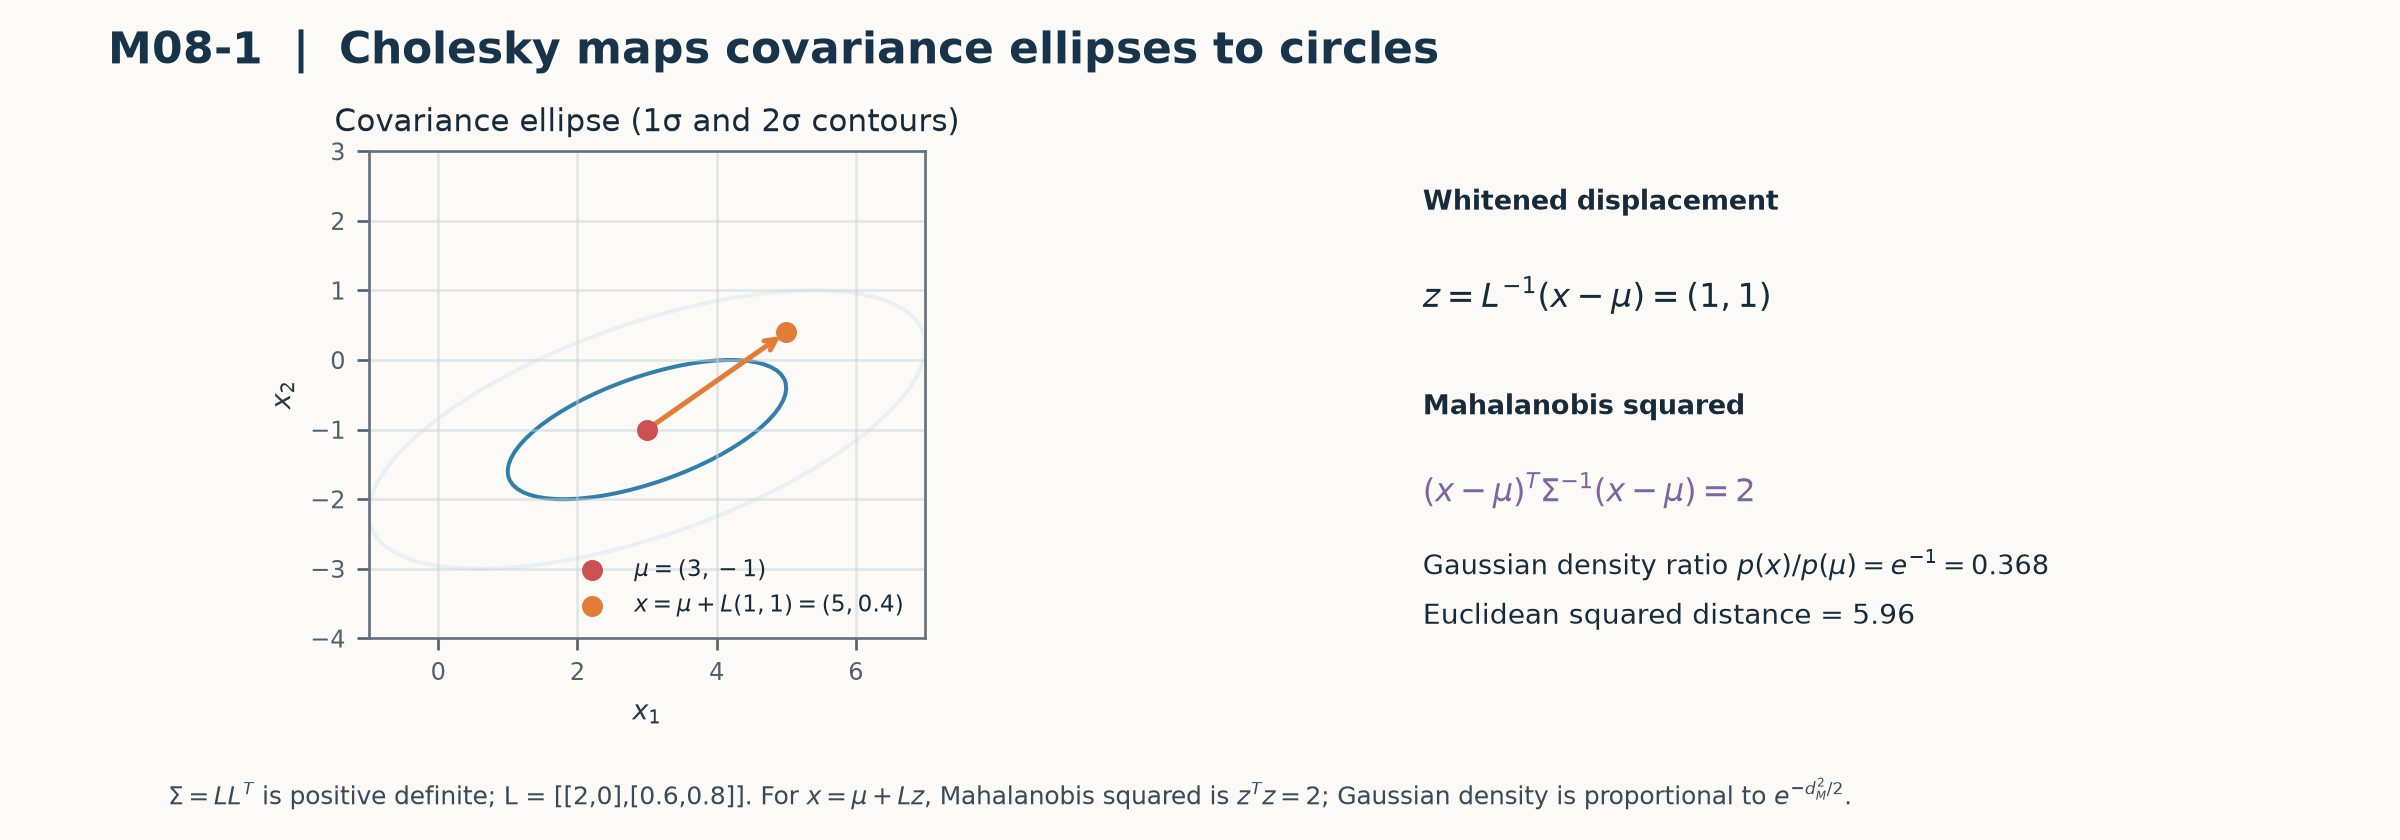
\includegraphics[keepaspectratio,alt={Visual Recall/Math Foundations/M08-1\_cholesky-whitening.png}]{Visual Recall/Math Foundations/M08-1_cholesky-whitening.png}}
\caption{Visual Recall/Math Foundations/M08-1\_cholesky-whitening.png}
\end{figure}

\textbf{M08-1. A covariance ellipse and its whitened coordinates.} For Sigma=\url{4,1.2\%5D,\%5B1.2,1}, L=\url{2,0\%5D,\%5B0.6,0.8}, mu=(3,-1), z=(1,1), x=(5,0.4), Mahalanobis squared distance 2, Euclidean squared distance 5.96, and density exp(-1)/(3.2 pi), about 0.0366 for an SPD 2D Gaussian.
